% =======================================================================================
\section{Comparison with MCMC}
\label{app:mcmc}
% =======================================================================================
% STATUS (2026-10-11): filled; windows q0.30 and q0.80 added (research log F28). lisa_checks/mcmc_xs.py (jexplore, needs .venv313) ran on a laptop
% GPU, two seeds per window; lisa_checks/compare_mcmc.py makes the per-window summaries, which
% scripts/import_data.py mcmc copies into data/mcmc. Tables from scripts/tables.py, the figure
% from scripts/fig_mcmc.py. Research log F27.

\subsection{MCMC for Galactic Binaries}

The standard analysis of LISA's galactic binaries is a global fit
\citep{cornish2007tests,littenberg2020global,littenberg2023prototype,strub2024global,katz2024efficient,deng2025modular}:
a Markov chain samples all resolvable sources at once, together with the noise, moves
between models with different numbers of sources by reversible jumps
\citep{green1995reversible}, and uses parallel tempering
\citep{earl2005parallel,vousden2016dynamic} to cross between the modes of
\cref{app:priors-symmetries}. The frequency band is split into overlapping segments
that are updated in turn, which is what makes the problem tractable and is also the unit our
windows imitate. Each new stretch of data, or each change of the noise model, means sampling
again. An amortised posterior estimator costs one forward integration per window once
trained, which is what makes it attractive as a proposal distribution, as a fast first pass, or
for population studies that need many independent analyses.
Normalising flows have been proposed as priors and proposals for these samplers
\citep{korsakova2024neural,sasli2026learned}, and sequential Monte Carlo parallelises their
trans-dimensional moves \citep{demasi2026massively}. Amortised posteriors for one or two
binaries have been compared with MCMC by \citet{delmond2026neural}, and slot-based posteriors
of sinusoidal mixtures with RJMCMC by \citet{houba2025slotflow} (\cref{app:related}).

\subsection{Sampler}

Our reference sampler is \texttt{jexplore}, a JAX parallel-tempered ensemble MCMC developed in
the LISA community, with affine-invariant stretch moves \citep{goodman2010ensemble,foreman2013emcee} and temperature swaps, run on the likelihood of \cref{eq:loglik} and the
priors of \cref{tab:prior}. For one source (8 dimensions), 32 walkers at four temperatures
(1, 1.6, 2.56, 4.1) for 20\,000 iterations, the second half kept, take about a minute on a GPU,
with acceptance rates of 0.24 (stretch) and 0.32 (swap) and $\hat R<1.0002$. On a published
source, this sampler on our likelihood reproduces the published posterior
(\cref{app:noise-validation}).

For the four-source windows below, the sampler runs on all 32 parameters jointly. Each source
is sampled as $(\ln f_0, \ln\Mc, \ln\Amp, \alpha, \sin\delta, \psi, \cos\iota, \phi_0)$ under the
training prior (\cref{tab:prior}), with the likelihood in double precision. The three angles are
sampled on $2\pi$ intervals centred on their true values. That is a full period, so the prior
is unchanged, and no narrow mode is cut by an edge. The chirp-mass prior has no closed form, so
we compute its density by quadrature over the primary mass. It matches $2\times10^6$ prior
draws ($\chi^2/\text{dof}=0.72$ over 60 bins).

Each iteration is a temperature swap, followed by either a differential-evolution or a stretch
move, with equal probability. There are 64 walkers at each of six temperatures from 1 to 10.
The walkers start from the window's Fisher draws, with chirp masses drawn from the prior. We
discard 100\,000 iterations and keep 300\,000, thinned by 100, and run each window twice with
independent seeds.

\subsection{Flow against MCMC}

\paragraph{Protocol.}
Four XS eval windows, named by their quantile in window SNR (\cref{app:evaluation}). The first
two probe the two limitations of \cref{app:xs}; the last two were added to test the flow's
misses, since each holds a faint or moderate source within 0.21 bins of a loud one:
\begin{itemize}
  \item q1.00, the loudest (window SNR 1848, sources at SNR 14, 33, 1245 and 1366), where the
        $f_0$ floor and the amplitude--inclination width matter;
  \item q0.60, the crowded window of \cref{fig:corner-median} (SNR 26, 27, 62 and 567), where
        the flow misses an SNR-27 source;
  \item q0.30 (SNR 9.1, 37, 111 and 235), with the SNR-37 source 0.16 bins from the SNR-235
        one;
  \item q0.80 (SNR 9.3, 9.5, 64 and 819), with an SNR-9.3 source 0.21 bins from the SNR-819
        one and the SNR-64 source 1.1 bins from it.
\end{itemize}
For each window, the MCMC uses the same noise realisation as the flow. We relabel its samples
as the flow's (\cref{app:evaluation-matching}), and fold $\psi$ and $\phi_0$ of both sample
sets by the exact symmetries of \cref{eq:psi-phi-symmetry} before comparing. For all eight
parameters we then compare:
\begin{itemize}
  \item the marginal widths ($1.4826\,\MAD$);
  \item the 1-D Wasserstein distances, in units of the MCMC width;
  \item the coverage of the MCMC medians by the flow's intervals.
\end{itemize}

\paragraph{The MCMC is converged, and Fisher holds in $f_0$.}
\Cref{tab:mcmc-checks} checks the sampler itself.
\begin{itemize}
  \item The two seeds agree within 7.5\% in every width and within $0.1\sigma$ in $W_1$. The
        exceptions are the SNR-14 source ($0.49\sigma$), whose sky posterior is broad and
        multimodal, and an SNR-9.3 source ($0.22\sigma$).
  \item In $f_0$ the Fisher forecast matches the MCMC within 3\% for every source at SNR
        $\ge62$, and within 16\% below. So the ``$\times$ ideal'' of \cref{app:xs} compares the
        flow with the true posterior where the floor is quoted.
  \item In the other parameters the forecast is within a factor 0.8--1.4 for most sources, but
        it can be off by up to 2.5 at SNR $\lesssim60$, by 1.9 for the SNR-235 source, and by up to 4.5 for the nearly face-on
        SNR-819 source of q0.80 ($\cos\iota = 0.995$), where the linearised forecast spreads
        along the $(\psi,\phi_0)$ and amplitude--inclination degeneracies that the true
        posterior bounds.
\end{itemize}

\begin{table}[h]
\caption{The MCMC itself, per source: its $f_0$ width, the Fisher forecast against it, and the
two seeds against each other. ``Other'' spans the six parameters besides $f_0$ and the
prior-dominated $\Mc$. The seed columns are maxima over the eight parameters: of
$|$width ratio $-1|$, and of $W_1$ in units of the MCMC width.}
\label{tab:mcmc-checks}
\centering
\small
% generated by paper/scripts/tables.py from data/mcmc; do not edit by hand
\begin{tabular}{lrccccc}
\toprule
& & MCMC $f_0$ & \multicolumn{2}{c}{width, Fisher / MCMC} & \multicolumn{2}{c}{seed 1 against seed 0} \\
\cmidrule(lr){4-5} \cmidrule(lr){6-7}
window & SNR & width [bins] & $f_0$ & other & max $|$width ratio $-1|$ & max $W_1/\sigma$ \\
\midrule
q1.00 & 1365.6 & 0.00045 & 0.98 & 0.81--1.39 & 0.031 & 0.04 \\
q1.00 & 1245.4 & 0.00056 & 0.98 & 0.79--1.04 & 0.075 & 0.10 \\
q1.00 & 32.9 & 0.016 & 1.03 & 0.93--1.42 & 0.042 & 0.05 \\
q1.00 & 14.4 & 0.046 & 0.93 & 0.40--0.99 & 0.057 & 0.49 \\
\midrule
q0.60 & 567.4 & 0.0013 & 0.98 & 0.92--1.05 & 0.020 & 0.02 \\
q0.60 & 62.4 & 0.0097 & 0.99 & 0.49--1.27 & 0.013 & 0.02 \\
q0.60 & 27.1 & 0.023 & 1.06 & 0.67--1.12 & 0.012 & 0.02 \\
q0.60 & 26.3 & 0.023 & 0.95 & 0.93--1.07 & 0.012 & 0.01 \\
\midrule
q0.30 & 235.1 & 0.0031 & 0.97 & 0.93--1.87 & 0.016 & 0.01 \\
q0.30 & 111.1 & 0.0052 & 0.98 & 1.00--1.29 & 0.014 & 0.02 \\
q0.30 & 37.2 & 0.018 & 1.09 & 1.15--1.74 & 0.028 & 0.02 \\
q0.30 & 9.1 & 0.07 & 0.87 & 0.45--1.21 & 0.014 & 0.03 \\
\midrule
q0.80 & 818.8 & 0.00088 & 1.01 & 0.99--4.51 & 0.043 & 0.03 \\
q0.80 & 63.8 & 0.011 & 1.02 & 0.98--1.03 & 0.031 & 0.03 \\
q0.80 & 9.5 & 0.071 & 0.84 & 0.72--1.25 & 0.030 & 0.06 \\
q0.80 & 9.3 & 0.069 & 1.13 & 0.44--2.40 & 0.027 & 0.22 \\
\bottomrule
\end{tabular}

\end{table}

\paragraph{Flow against MCMC.}
\Cref{tab:mcmc} gives the width ratios, and \cref{fig:mcmc} the loudest source.
\begin{itemize}
  \item \textbf{Not biased.} The MCMC median lies inside the flow's central 95\% interval for
        127 of the 128 source--parameter pairs, and inside its 68\% interval for 112. The
        exception is the sky latitude of an SNR-9.3 source that the flow misses. Where the
        flow finds a source it is conservative, as the coverage of \cref{app:xs} said.
  \item \textbf{Loud sources are too wide in every measured parameter.} In $f_0$ the flow is 6.4, 11,
        38, 44, 66 and 84 times the MCMC width at SNR 111, 235, 567, 819, 1245 and 1366: a
        width that stays near the floor of \cref{app:xs} while the MCMC's falls as
        $1/\snr$. The sky, amplitude, inclination and the two phases are 3--8.5 times too wide
        above SNR 500. The MCMC follows the same curved amplitude--inclination degeneracy as
        the flow (\cref{fig:mcmc}), but is four times narrower along it. So the flow's excess
        width there is not a non-Gaussianity that the Fisher forecast misses, and the
        precision limit is not specific to $f_0$, though $f_0$ is where it costs most.
  \item \textbf{Moderate sources, once found, are near-optimal when isolated.} At SNR 26--33
        the flow is within 1.0--2.1 times the MCMC in every parameter but $f_0$ (2.3--4.8),
        and at SNR 111 within 1.8--2.6. An SNR-64 source 1.1 bins from the SNR-819 one is
        the exception: 6--11 times too wide in every parameter but $f_0$ (19), with 8\% of its draws
        relabelled off it.
  \item \textbf{The flow misses six of the sixteen sources, and the data do not.} The MCMC
        localises every source, in $f_0$ as the Fisher forecast predicts (\cref{tab:mcmc-checks}),
        while most of the flow's draws for the missed ones are more than a bin away (56--89\%).
        Five of the six sit within 2.6 bins of a source 6 to 90 times louder: SNR 14 next to
        1245, 27 next to 567, 37 next to 235 (at 0.16 bins), 9.1 next to 111 and 9.3 next to
        819; the sixth, at SNR 9.5, is 4.9 bins from the other SNR-9 source. When one slot does
        not lock on, the relabelling of \cref{app:evaluation-matching} can hand a brighter
        neighbour's slot to the missed source in up to a fifth of the draws (SNR 33 and 62),
        although almost every draw has a slot on the brighter source. The scorecard shows the same pattern over 840 sources: detection falls
        with the distance to the nearest source, most of all next to a louder one
        (\cref{tab:xs-separation}).
  \item $\psi$ and $\phi_0$ of two nearly face-on sources ($\cos\iota=0.98$ at SNR 62 and
        $0.87$ at SNR 235) are constrained mostly in a combination, in both methods, so
        the ratio of their separate widths (0.45--0.5) means little. The chirp mass is
        prior-dominated in both (ratios 0.92--1.06).
\end{itemize}

\begin{table}[h]
\caption{Flow against MCMC on the four windows: ratio of marginal widths (flow / MCMC) per
parameter, after relabelling and folding $\psi$ and $\phi_0$ by their exact symmetries. The
last column is the share of the flow's draws more than a bin from the MCMC median in $f_0$.
In every entry but the one marked $^\ast$ (the sky latitude) the MCMC median lies inside the
flow's central 95\%.}
\label{tab:mcmc}
\centering
\small
% generated by paper/scripts/tables.py from data/mcmc; do not edit by hand
\begin{tabular}{lrccccccccr}
\toprule
& & \multicolumn{8}{c}{width, flow / MCMC} & off \\
\cmidrule(lr){3-10}
window & SNR & $f_0$ & $\Mc$ & $\Amp$ & $\alpha$ & $\sin\delta$ & $\psi$ & $\cos\iota$ & $\phi_0$ & $>1$ bin \\
\midrule
q1.00 & 1365.6 & 84 & 0.95 & 4.21 & 5.44 & 5.72 & 6.62 & 4.29 & 6.62 & 0\% \\
q1.00 & 1245.4 & 66 & 1.06 & 3.62 & 6.37 & 6.41 & 8.42 & 3.86 & 8.39 & 0\% \\
q1.00 & 32.9 & 4.78 & 0.95 & 1.36 & 1.76 & 2.06 & 1.06 & 2.11 & 1.03 & 20\% \\
q1.00 & 14.4 & 21 & 0.97 & 5.14 & 4.09 & 5.41 & 2.04 & 8.38 & 9.51 & 58\% \\
\midrule
q0.60 & 567.4 & 38 & 0.99 & 4.81 & 5.75 & 4.47 & 5.00 & 4.11 & 4.76 & 0\% \\
q0.60 & 62.4 & 6.24 & 1.02 & 2.58 & 6.76 & 3.77 & 0.47 & 1.71 & 0.53 & 18\% \\
q0.60 & 27.1 & 231 & 1.01 & 4.45 & 54 & 34 & 2.77 & 3.66 & 5.59 & 87\% \\
q0.60 & 26.3 & 2.30 & 1.04 & 1.03 & 1.12 & 1.20 & 1.17 & 1.08 & 1.15 & 0\% \\
\midrule
q0.30 & 235.1 & 11 & 0.96 & 1.82 & 4.35 & 3.23 & 0.47 & 1.57 & 0.45 & 0\% \\
q0.30 & 111.1 & 6.37 & 1.00 & 2.64 & 2.44 & 1.81 & 2.26 & 2.61 & 2.33 & 0\% \\
q0.30 & 37.2 & 154 & 1.02 & 3.68 & 11 & 9.29 & 3.56 & 5.27 & 6.86 & 64\% \\
q0.30 & 9.1 & 52 & 0.92 & 1.53 & 4.86 & 24 & 1.02 & 2.17 & 1.96 & 56\% \\
\midrule
q0.80 & 818.8 & 44 & 1.05 & 3.00 & 8.45 & 8.48 & 4.51 & 2.98 & 4.51 & 0\% \\
q0.80 & 63.8 & 19 & 0.98 & 8.14 & 6.36 & 9.02 & 9.34 & 8.01 & 11 & 8\% \\
q0.80 & 9.5 & 46 & 0.97 & 3.75 & 19 & 4.90 & 2.75 & 2.72 & 4.87 & 89\% \\
q0.80 & 9.3 & 45 & 0.97 & 4.02 & 1.90 & 35$^\ast$ & 0.91 & 2.51 & 1.23 & 81\% \\
\bottomrule
\end{tabular}

\end{table}

\paragraph{With position features.}
\Cref{tab:mcmc-r1} repeats the comparison for the model with position features (R1,
\cref{app:b}), on the same windows and data, with its eval draws regenerated from the same keys.
\begin{itemize}
  \item \textbf{The frequency is fixed.} Loud sources are now 5--12 times the MCMC width in
        $f_0$ instead of 38--84, and found moderate ones (SNR 26--235) 1.2--3.0 times. The
        exception is the crowded SNR-64 source (19 times), 1.1 bins from the SNR-819 one.
  \item \textbf{The other parameters are not.} The amplitude, sky, inclination and phases of the
        loud sources stay 3--9 times too wide, and 12 times for the crowded SNR-64 one. So the
        features remove the precision limit of the frequency coordinate, not that of the others.
  \item \textbf{The same six sources are missed.}
  \item \textbf{Coverage.} With narrower posteriors, three of the 128 entries fall outside the
        flow's 95\% interval (125 of 128; 108 inside the 68\%). One is the sky latitude of the
        missed SNR-9.3 source, as before. The other two are the amplitude and longitude of the
        SNR-235 source in q0.30, shifted by 3 and 8 MCMC widths ($W_1$). That source sits 0.16
        bins from the missed SNR-37 one, and the flow assigns part of the neighbour's signal to
        it. A missed neighbour biases its loud companion, by an amount the wider posteriors
        without the features covered and the sharper ones no longer do.
\end{itemize}

\begin{table}[h]
\caption{Flow against MCMC for the final model and for R1 (position features), on the four
windows. Width ratios (flow / MCMC) in $f_0$ and, as a median, over $\Amp$, the sky,
$\cos\iota$, $\psi$ and $\phi_0$; and the share of the flow's draws more than a bin from the MCMC
median in $f_0$. A star marks a source with a parameter whose MCMC median lies outside the
flow's central 95\%.}
\label{tab:mcmc-r1}
\centering
\small
% generated by paper/scripts/tables.py from data/mcmc; do not edit by hand
% R1: MCMC median inside the flow's 95%: 125/128, 68%: 108/128
\begin{tabular}{lrcccccc}
\toprule
& & \multicolumn{2}{c}{$f_0$, flow / MCMC} & \multicolumn{2}{c}{other, median} & \multicolumn{2}{c}{off $>1$ bin} \\
\cmidrule(lr){3-4} \cmidrule(lr){5-6} \cmidrule(lr){7-8}
window & SNR & final & R1 & final & R1 & final & R1 \\
\midrule
q1.00 & 1365.6 & 84 & 7.3 & 5.6 & 6.5 & 0\% & 0\% \\
q1.00 & 1245.4 & 66 & 5.3 & 6.4 & 6.5 & 0\% & 0\% \\
q1.00 & 32.9 & 4.8 & 1.8 & 1.6 & 1.4 & 20\% & 23\% \\
q1.00 & 14.4 & 21 & 45 & 5.3 & 7.8 & 58\% & 71\% \\
\midrule
q0.60 & 567.4 & 38 & 5.0 & 4.8 & 5.8 & 0\% & 0\% \\
q0.60 & 62.4 & 6.2 & 3.0 & 2.1 & 2.3 & 18\% & 18\% \\
q0.60 & 27.1 & 231 & 248 & 5.0 & 4.9 & 87\% & 84\% \\
q0.60 & 26.3 & 2.3 & 1.2 & 1.1 & 1.2 & 0\% & 0\% \\
\midrule
q0.30 & 235.1 & 11 & 2.5$^\ast$ & 1.7 & 1.2 & 0\% & 0\% \\
q0.30 & 111.1 & 6.4 & 1.4 & 2.4 & 2.0 & 0\% & 0\% \\
q0.30 & 37.2 & 154 & 330 & 6.1 & 5.6 & 64\% & 81\% \\
q0.30 & 9.1 & 52 & 145 & 2.1 & 2.3 & 56\% & 70\% \\
\midrule
q0.80 & 818.8 & 44 & 12 & 4.5 & 3.2 & 0\% & 0\% \\
q0.80 & 63.8 & 19 & 19 & 8.6 & 12 & 8\% & 14\% \\
q0.80 & 9.5 & 46 & 53 & 4.3 & 4.1 & 89\% & 89\% \\
q0.80 & 9.3 & 45$^\ast$ & 47$^\ast$ & 2.2 & 2.2 & 81\% & 84\% \\
\bottomrule
\end{tabular}

\end{table}

\begin{figure}[h]
  \centering
  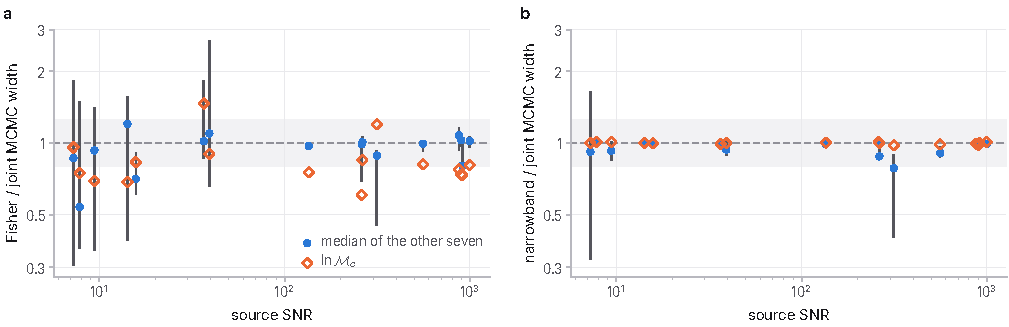
\includegraphics[width=0.92\textwidth]{figures/mcmc.pdf}
  \caption{The loudest eval source (SNR 1366, window at 0.1009\,mHz): the flow (blue), a joint
  MCMC of the window's four sources (black), the Fisher forecast (grey, dashed) and the truth
  (red). Contours enclose 39\% and 86\% of the mass. The MCMC draws are moved at random to
  the four exact $(\psi,\phi_0)$ copies, to show them on the flow's footing. MCMC and Fisher
  agree. The flow covers both, but is 4--8 times wider in every parameter but the
  prior-dominated $\Mc$, and 84 times wider in
  $f_0$.}
  \label{fig:mcmc}
\end{figure}

\paragraph{Cost.}
Once trained, the flow draws 256 posterior samples of an XS window in about a second on an
A100, and of a B window in about 42 seconds. The MCMC of one XS window takes 14--18 minutes
per seed on a laptop GPU: 400\,000 iterations of 384 chains with a double-precision
likelihood.
Training costs about 20 A100-hours on XS and 86 on B, paid once.
